\documentclass[12pt]{article}
\usepackage[utf8]{inputenc}
\usepackage[automark]{scrlayer-scrpage}
\usepackage[T1]{fontenc}
\usepackage[pdftex]{graphicx,color}
\usepackage{subcaption}
\usepackage{url}
\usepackage[pdftex,pdfpagelabels]{hyperref}
\usepackage[section,boxed]{algorithm}
\usepackage{algpseudocode}
\usepackage{amsmath}
\usepackage{amssymb}
\usepackage{amsthm}
\usepackage{lmodern}
\pagestyle{scrheadings}
\ofoot{}\cfoot{}\ifoot{}
\lehead{\pagemark}
\rehead{\slshape\leftmark}
\lohead{\slshape\leftmark}
\rohead{\pagemark}
\newtheorem{definition}{Definition}
\newtheorem{theorem}{Theorem}
\usepackage{blindtext}
\usepackage[ngerman]{babel}
\usepackage[margin=1in]{geometry}
\usepackage{amsmath,amsthm,amssymb}
\usepackage{graphicx}
\newcommand{\N}{\mathbb{N}}
\newcommand{\Z}{\mathbb{Z}}
\newcommand{\R}{\mathbb{R}}
\newcommand{\C}{\mathbb{C}}

\begin{document}
% --------------------------------------------------------------
%                         Title Page
% --------------------------------------------------------------
\title{Solutions for Sheet 3}
\author{Raphael Wude, Martin Brückmann, Claude Jordan, Daniel Degenstein\\ \\
\textsc{Pattern Matching and Machine Learning} \\
\textsc{for Audio Signal Processing}}
\maketitle

% --------------------------------------------------------------
%                         Task 1.1
% --------------------------------------------------------------
\section*{Task 3.1}
\begin{itemize}
    \item[(a)] We have the following formulas for $cos(z)$ and $u_k$:
    \begin{align*}
      cos(z) &= \frac{1}{2} e^{iz} + e^{-iz} \\
      u_k &= e^{\frac{2 \pi i k n}{N}}
    \end{align*}
    So for f, we get:
    \begin{align*}
      f(t) &= cos(4\pi t) + 4 cos(20\pi t) + 8 cos(2\pi 20 t) = cos(2\pi 2 t) + 4 cos(2\pi 10 t) + 8 cos(2\pi 20 t)\\
      &= \frac{1}{2} \left( e^{2 \pi 2 t i} + e^{-2 \pi 2 t i} \right) + \frac{4}{2} \left( e^{2 \pi 10 t i} + e^{-2 \pi 10 t i} \right) + \frac{8}{2} \left( e^{2 \pi 20 t i} + e^{-2 \pi 20 t i} \right)\\
      &= \frac{1}{2} \left( e^{2 \pi 2 t i} + e^{-2 \pi 2 t i} \right) + 2 \left( e^{2 \pi 10 t i} + e^{-2 \pi 10 t i} \right) + 4 \left( e^{2 \pi 20 t i} + e^{-2 \pi 20 t i} \right)
    \end{align*}
    With $t=\frac{k}{N}$ we get:
    \begin{align*}
      f = \frac{1}{2} \left(u_2 + u_{N-2} \right) + 2 \left( u_{10} + u_{N-10} \right) + 4 \left(u_{20} + u_{N-20} \right)
    \end{align*}
      \item[(b)] We obtain from f:
      \begin{align*}
        |\hat f(k)|=w_k \cdot \frac{N}{2}
      \end{align*}
      with $w_2=w_{N-2}=1$, $w_{10}=w_{N-10}=2$, $w_{20}=w_{N-20}=4$ and otherwise $w_k=0$.
      \item[c)]
      \begin{figure}[H]
          \centering
          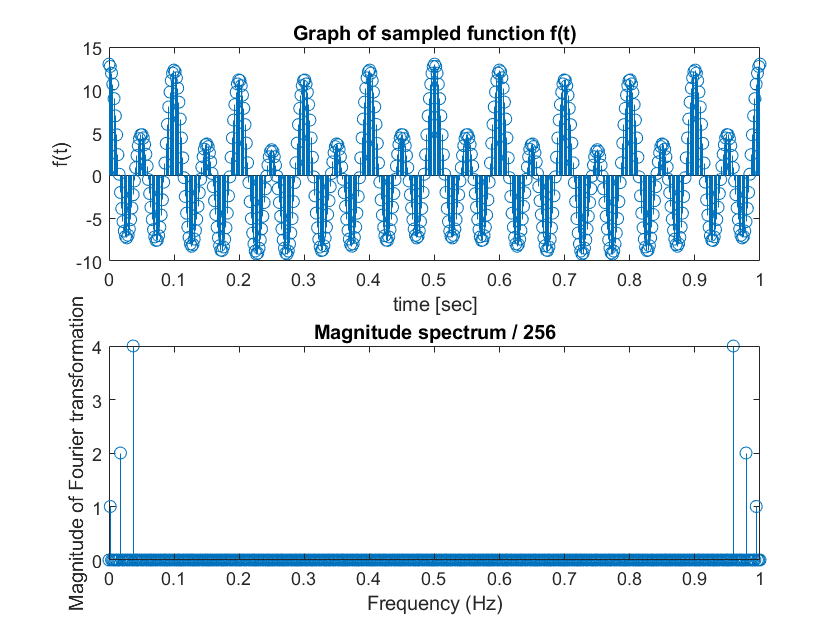
\includegraphics[width=1.1\textwidth]{Sheet3Exercise1.png}
          \caption{$f(t) (top) and |\hat f(k)| (bottom)$}
          \label{abb}
      \end{figure}
\end{itemize}

\end{document}
